% Текущая постановка: одна фиксированная среда, k in [1,2], три метода.
% Источники чисел: evidence/current_static_low/ и prepare_predictions.py.
\documentclass[notitle]{sibjima_preview}
\setlength{\paperwidth}{205mm}
\setlength{\paperheight}{290mm}
\AtBeginDvi{\special{papersize=205mm,290mm}}
\usepackage{fontspec}
\setmainfont{cmunrm.otf}[BoldFont=cmunbx.otf,ItalicFont=cmunti.otf,BoldItalicFont=cmunbi.otf]
\usepackage{booktabs,array,needspace}
\usepackage[hidelinks,unicode]{hyperref}
\hypersetup{pdftitle={Нейросетевое приближение рассеянного поля при фиксированной среде},pdfsubject={SVD-SNO, FNO и Chebyshev-SNO}}
\AddToHook{cmd/section/before}{\Needspace{7\baselineskip}}
\AddToHook{cmd/subsection/before}{\Needspace{6\baselineskip}}
\makeatletter
\setlength{\@fptop}{0pt}
\setlength{\@fpsep}{20pt}
\setlength{\@fpbot}{0pt plus 1fil}
\makeatother
\newcommand{\ii}{\mathrm{i}}
\newcommand{\R}{\mathbb{R}}
\newcommand{\C}{\mathbb{C}}
\newcommand{\trans}{\mathsf{T}}
\begin{document}
\thispagestyle{plain}
\pagestyle{plain}
\begin{center}
{\bfseries Нейросетевое приближение рассеянного поля при фиксированной среде: SVD-SNO, FNO и Chebyshev-SNO}
\end{center}

\textbf{Аннотация.}
Рассматривается двумерная задача рассеяния плоской волны на трёх проницаемых круговых включениях с фиксированными коэффициентами материала. По волновому числу и направлению волны предсказывается комплексное рассеянное поле на заданной конечно-элементной сетке. Сопоставляются SVD-SNO с модами, найденными по снимкам решения, FNO с преобразованиями Фурье и Chebyshev-SNO с фиксированным полиномиальным представлением. Для 1000 частот из диапазона \(k\in[1,2]\) и восьми направлений на каждую частоту сформированы 8000 FEM-полей. Разбиение выполняется по частотам: все направления одной частоты относятся к одной части выборки. На 1280 тестовых полях средние ошибки относительно FEM-меток в согласованной комплексной норме \(L^2\) составили 0,9475\% для SVD-SNO, 1,6599\% для FNO и 7,9364\% для Chebyshev-SNO. Выход SVD-SNO использует по десять POD-мод для действительной и мнимой частей. Для Chebyshev-SNO при \(8\times8\) модах средняя оптимальная ошибка её фиксированного декодера на валидации равна 7,6143\%. Результаты относятся к удержанным частотам одного материала и одному seed; точность относительно непрерывной задачи отдельно не установлена.

\textbf{Ключевые слова:} уравнение Гельмгольца; рассеяние волн; метод конечных элементов; POD; спектральный нейрооператор; FNO; полиномы Чебышёва.

\section{ВВЕДЕНИЕ}
При фиксированной среде серия задач рассеяния различается частотой и направлением падающей волны. FEM-решение каждой задачи даёт дискретную опорную метку, а заранее обученная сеть может приближать зависимость поля от параметров волны. Цель данной работы --- сопоставить три представления этого отображения на одном наборе данных и явно отделить точность выходного пространства от точности предсказания его коэффициентов.

В FNO обучаемая спектральная ветвь использует преобразование Фурье, а нелинейность действует на пространственные признаки~\cite{li2020}. В SNO функции представлены коэффициентами рядов, и сеть преобразует эти коэффициенты~\cite{fanaskov2022}. Здесь рассматриваются два coefficient-space варианта: SVD-SNO с POD-модами, найденными по FEM-снимкам, и Chebyshev-SNO с заранее заданными тензорными полиномами. Использование фиксированного POD-базиса для выходного поля известно также из POD-DeepONet~\cite{lu2022}; приведённая ниже SVD-SNO имеет собственную формулу блока и не объявляется воспроизведением этой архитектуры.

Материал одинаков для всех примеров. Поэтому фактически изучается конечнопараметрическое отображение
\begin{equation}
\mathcal G_h:(k,\theta)\longmapsto u_{s,h}(\cdot;k,\theta),
\qquad k\in[1,2],\quad \theta\in[0,2\pi).
\label{eq:mapping}
\end{equation}
Обозначения SNO и FNO описывают способ представления и обработки поля. Тест не проверяет новые материалы, геометрии или сетки. Для воспроизводимого сопоставления фиксируются FEM-метрика, групповые индексы, настройки моделей и сохранённые веса.

\section{ЗАДАЧА РАССЕЯНИЯ И FEM-МЕТКИ}
Пусть \(\Omega=(-2,2)^2\), а падающая волна равна
\begin{equation}
u_i(\bm x)=\exp(\ii k\bm d\cdot\bm x),\qquad
\bm d=(\cos\theta,\sin\theta).
\label{eq:incident}
\end{equation}
Вещественные скалярные коэффициенты \(A>0\) и \(n>0\) постоянны внутри каждого круга; вне включений \(A=n=1\). Таблица~\ref{tab:material} задаёт используемый материал. Координаты и коэффициенты округлены для чтения; расчёты используют исходные DG0-массивы. Геометрия показана на рис.~\ref{fig:medium}.

\begin{table}[htbp]
\centering
\caption{Одна фиксированная среда во всех обучающих и тестовых примерах}
\label{tab:material}
\begin{tabular}{@{}rrrrr@{}}
\toprule
\(x_c\) & \(y_c\) & Радиус & \(A\) & \(n\)\\
\midrule
\(-0,6\) & \(0,1\) & \(0,05\) & 0,69286575 & 2,59454354\\
\(0,4\) & \(0\) & \(0,10\) & 0,86604243 & 1,69621106\\
\(-0,3\) & \(-0,3\) & \(0,05\) & 0,78180951 & 1,84454536\\
\bottomrule
\end{tabular}
\end{table}

\begin{figure}[htbp]
\centering
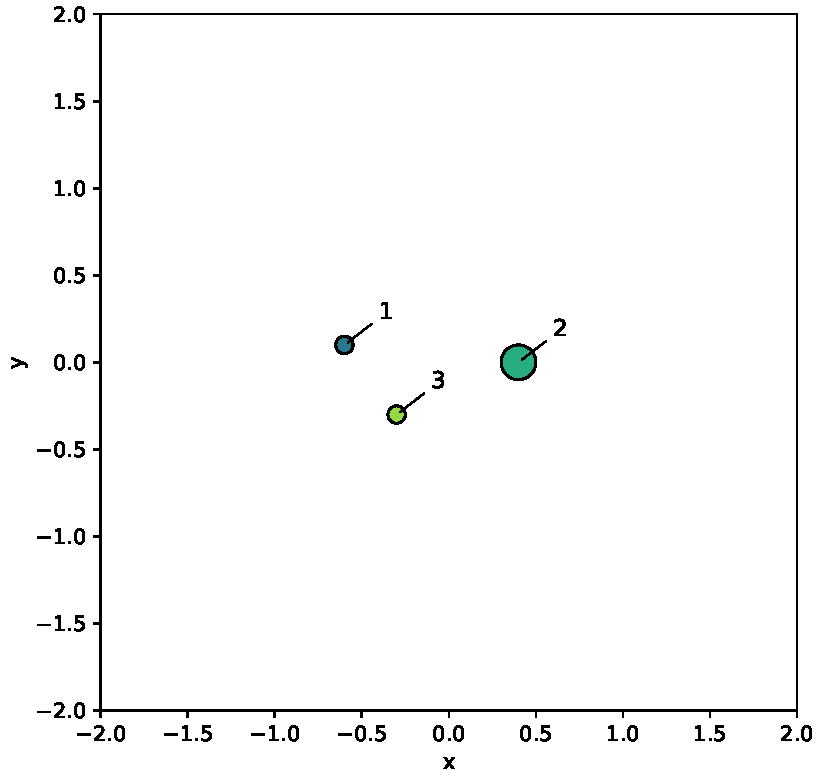
\includegraphics[width=0.48\linewidth]{images/static_medium_geometry.pdf}
\caption{Расчётная область и три активных включения. Цвет выделяет материальные области; нумерация соответствует строкам табл.~\ref{tab:material}.}
\label{fig:medium}
\end{figure}

Полное поле \(u=u_i+u_s\) удовлетворяет уравнению \(\nabla\cdot(A\nabla u)+k^2nu=0\). Для рассеянного поля
\begin{equation}
\nabla\cdot(A\nabla u_s)+k^2nu_s
=\nabla\cdot\bigl((1-A)\nabla u_i\bigr)+k^2(1-n)u_i.
\label{eq:helmholtz}
\end{equation}
На внешней границе задаётся локальное поглощающее условие первого порядка
\begin{equation}
A\partial_\nu u_s-\ii ku_s=0.
\label{eq:boundary}
\end{equation}
Все включения расположены внутри области; вблизи границы \(A=n=1\). Условие~\eqref{eq:boundary} задаёт ограниченную задачу с приближением излучения на конечном квадрате.

Пусть \(V_h\subset H^1(\Omega;\C)\) --- пространство непрерывных кусочно-линейных функций. Найти \(u_{s,h}\in V_h\), такое, что для любого \(v_h\in V_h\)
\begin{equation}
\begin{aligned}
&\int_\Omega A\nabla u_{s,h}\cdot\nabla\overline{v_h}\,d\bm x
-k^2\int_\Omega nu_{s,h}\overline{v_h}\,d\bm x
-\ii k\int_{\partial\Omega}u_{s,h}\overline{v_h}\,ds\\
&\qquad=-\int_\Omega(A-1)\nabla u_i\cdot\nabla\overline{v_h}\,d\bm x
+k^2\int_\Omega(n-1)u_i\overline{v_h}\,d\bm x.
\end{aligned}
\label{eq:weak}
\end{equation}
При скачках \(A\) правая часть учитывает интерфейсный вклад в слабом смысле. Подстановка только объёмного выражения по материалам не эквивалентна~\eqref{eq:weak}. При \(A=n=1\) правая часть обращается в нуль.

Общая согласованная треугольная сетка содержит 3221 узел и 6280 треугольников; целевой фоновый шаг равен \(h=0,1\). Решается комплексная система
\begin{equation}
\bigl(K(A)-k^2M(n)-\ii kM_{\partial\Omega}\bigr)\bm u_s=\bm b(k,\theta)
\label{eq:system}
\end{equation}
с использованием LU. Исходные материальные коэффициенты задаются на ячейках. Для входа пространственных сетей они усредняются в узлах по прилегающим элементам с равными весами; FEM-сборка использует исходные DG0-поля.

\section{ВЫБОРКА, НОРМИРОВКА И ОБЩАЯ МЕТРИКА}
Частоты расположены равномерно:
\begin{equation}
k_f=1+\frac{f}{999},\qquad f=0,\ldots,999.
\label{eq:frequencies}
\end{equation}
Для каждой частоты воспроизводимо выбирается сдвиг \(\theta_{0,f}\in[0,\pi/4)\) и восемь направлений
\(\theta_{f,j}=\theta_{0,f}+2\pi j/8\), \(j=0,\ldots,7\). Всего имеется 8000 комплексных полей. Частотные группы перемешиваются с seed 2026; все восемь направлений одной частоты остаются вместе.

\begin{table}[htbp]
\centering
\caption{Групповое разбиение одной среды}
\label{tab:split}
\begin{tabular}{@{}lrrl@{}}
\toprule
Выборка & Частоты & Поля & Назначение\\
\midrule
Обучающая & 670 & 5360 & Базисы, статистики, веса сети\\
Валидационная & 170 & 1360 & Выбор ранга и состояния сети\\
Тестовая & 160 & 1280 & Оценка зафиксированных моделей\\
\bottomrule
\end{tabular}
\end{table}

Средние, масштабы и POD-моды вычисляются только по train. Углы представлены парой \((\cos\theta,\sin\theta)\), а частота нормируется обучающими средним и стандартным отклонением. Все методы предсказывают два вещественных канала. После восстановления физических масштабов
\begin{equation}
\widehat u_s=\widehat u_{\rm re}+\ii\widehat u_{\rm im},\qquad
|\widehat u_s|=\sqrt{\widehat u_{\rm re}^2+\widehat u_{\rm im}^2}.
\label{eq:components}
\end{equation}
Модуль вычисляется из восстановленного поля, а не из модулей его коэффициентов.

Основная ошибка для каждого примера равна
\begin{equation}
e_M=\left(\frac{(\widehat{\bm u}-\bm u)^*M(\widehat{\bm u}-\bm u)}{\bm u^*M\bm u}\right)^{1/2}.
\label{eq:metric}
\end{equation}
Здесь \(M\) --- согласованная матрица массы для невзвешенной нормы \(L^2(\Omega)\), а не материальная \(M(n)\) из~\eqref{eq:system}. На треугольнике \(T\)
\begin{equation}
M_T=\frac{|T|}{12}\begin{pmatrix}2&1&1\\1&2&1\\1&1&2\end{pmatrix}.
\label{eq:mass}
\end{equation}
Это точная интеграция квадрата модуля P1-поля на данной сетке. Функция потерь --- среднее индивидуальных \(e_M\) по пакету. Табличные проценты получаются умножением соответствующих статистик индивидуальных ошибок на 100. Среднее ошибок не равно отношению суммарных норм всей выборки. Все результаты сравниваются с дискретным FEM-решением; отдельно точность непрерывной задачи не установлена.

\section{SVD-SNO: МОДЫ И ПРЕДСКАЗАНИЕ КОЭФФИЦИЕНТОВ}
\subsection{Взвешенный POD и выбор ранга}
Для каждого вещественного компонента \(f\in\{\operatorname{Re}u_s,\operatorname{Im}u_s\}\) обучающие снимки центрируются. Пусть \(F_c\in\R^{N_{\rm tr}\times N_h}\) содержит их по строкам, а \(\bm m\) --- обучающее среднее. При \(W=\operatorname{diag}(M\bm1)\) используется разложение
\begin{equation}
F_cW^{1/2}=U\Sigma V^\trans,\qquad
\Phi_r=W^{-1/2}V_r,\qquad \Phi_r^\trans W\Phi_r=I.
\label{eq:pod}
\end{equation}
Столбцы \(\Phi_r\) --- пространственные моды в FEM-узлах. Сингулярные значения упорядочивают их вклад в суммарную взвешенную изменчивость train-снимков. Коэффициенты и реконструкция задаются формулами
\begin{equation}
\bm c_W=\Phi_r^\trans W(\bm f-\bm m),\qquad
\bm f_r=\bm m+\Phi_r\bm c_W.
\label{eq:pod_encode}
\end{equation}
Разложение вычисляется рандомизированным алгоритмом~\cite{halko2011}: для предела 48 мод берутся десять дополнительных случайных направлений и две степенные итерации с промежуточной QR-ортогонализацией. После проекции на найденное подпространство SVD выполняется для меньшей матрицы. Это способ приближённого построения базиса, а не отдельная обучаемая сеть.

Из рангов до 48 выбирается первый общий ранг Re/Im, для которого средняя валидационная FEM-ошибка реконструкции не превышает 1\%. Получено \(r=10\). Для неизменных \(A,n\) центрированные матрицы снимков нулевые, поэтому их входные POD-ранги равны нулю. Отсутствующие моды не заменяются численным шумом: меняются только параметры волны.

Для каждой выходной моды сеть предсказывает нормированный коэффициент
\(\widetilde c_j=(c_j-\mu_j)/s_j\), где \(\mu_j,s_j\) определяются по train. При декодировании сначала возвращаются эти масштабы, затем прибавляется среднее поле. Матрица \(W\) используется только в построении и кодировании POD; итоговая ошибка остаётся~\eqref{eq:metric} с согласованной \(M\).

\subsection{Сеть версии 2: что означают Z, B и W}
Для полноты общий случай имеет \(R=\max(r_A,r_n,r)\) модальных позиций. Нормированные коэффициенты материалов дополняются нулями до \(R\), а параметры волны повторяются в каждой строке:
\begin{equation}
C_{j,:}=\bigl(\operatorname{pad}(\widetilde{\bm c}_A)_j,
\operatorname{pad}(\widetilde{\bm c}_n)_j,\cos\theta,\sin\theta,\widetilde k\bigr).
\label{eq:tokens}
\end{equation}
В текущем эксперименте \(R=r=10\), и первые два столбца равны нулю. Этот вход описывает параметры волны при заранее зафиксированном материале.

Общий линейный подъём и три остаточных блока имеют вид
\begin{equation}
\begin{aligned}
Z^{(0)}&=\sigma(CW_0+\bm1b_0^\trans),\\
Z^{(\ell+1)}&=Z^{(\ell)}+\sigma\!\left(
Z^{(\ell)}W_{\rm loc}^{(\ell)}+\bm1(b_{\rm loc}^{(\ell)})^\trans
+B^{(\ell)}Z^{(\ell)}W_{\rm ch}^{(\ell)}\right),\quad \ell=0,1,2.
\end{aligned}
\label{eq:sno_block}
\end{equation}
Здесь \(\sigma\) --- GELU; \(Z^{(\ell)}\in\R^{10\times24}\) содержит скрытые признаки одного запроса. Строки соответствуют модальным позициям, столбцы --- скрытым каналам. \(Z\) пересчитывается при изменении \(k,\theta\); верхний индекс означает номер слоя.

Матрицы \(B^{(\ell)}\in\R^{10\times10}\) и \(W_{\rm loc}^{(\ell)},W_{\rm ch}^{(\ell)}\in\R^{24\times24}\) --- обучаемые веса, фиксированные при предсказании. Умножение справа на \(W\) смешивает каналы одной строки, умножение слева на \(B\) --- модальные позиции одного канала:
\begin{equation}
(ZW)_{j,c}=\sum_dZ_{j,d}W_{d,c},\qquad
(BZ)_{j,c}=\sum_iB_{j,i}Z_{i,c}.
\label{eq:mixing}
\end{equation}
Матрица \(B\) не является пространственным POD-базисом \(\Phi\) или FEM-матрицей. Термин «локальная ветвь» означает обработку одной модальной строки; это не локальность в физической области.

Проекция \(24\to2\) даёт коэффициенты Re и Im, после денормировки
\begin{equation}
\widehat{\bm u}=\bm m_{\rm re}+\Phi_{\rm re}\widehat{\bm c}_{\rm re}
+\ii\bigl(\bm m_{\rm im}+\Phi_{\rm im}\widehat{\bm c}_{\rm im}\bigr).
\label{eq:decode}
\end{equation}
Общее число вещественных параметров равно
\begin{equation*}
(5\cdot24+24)+3(24^2+24+10^2+24^2)+(24\cdot2+2)=4022.
\end{equation*}
Веса сохраняют \texttt{architecture\_version=2}; схема приведена на рис.~\ref{fig:sno}.

\begin{figure}[p]
\centering
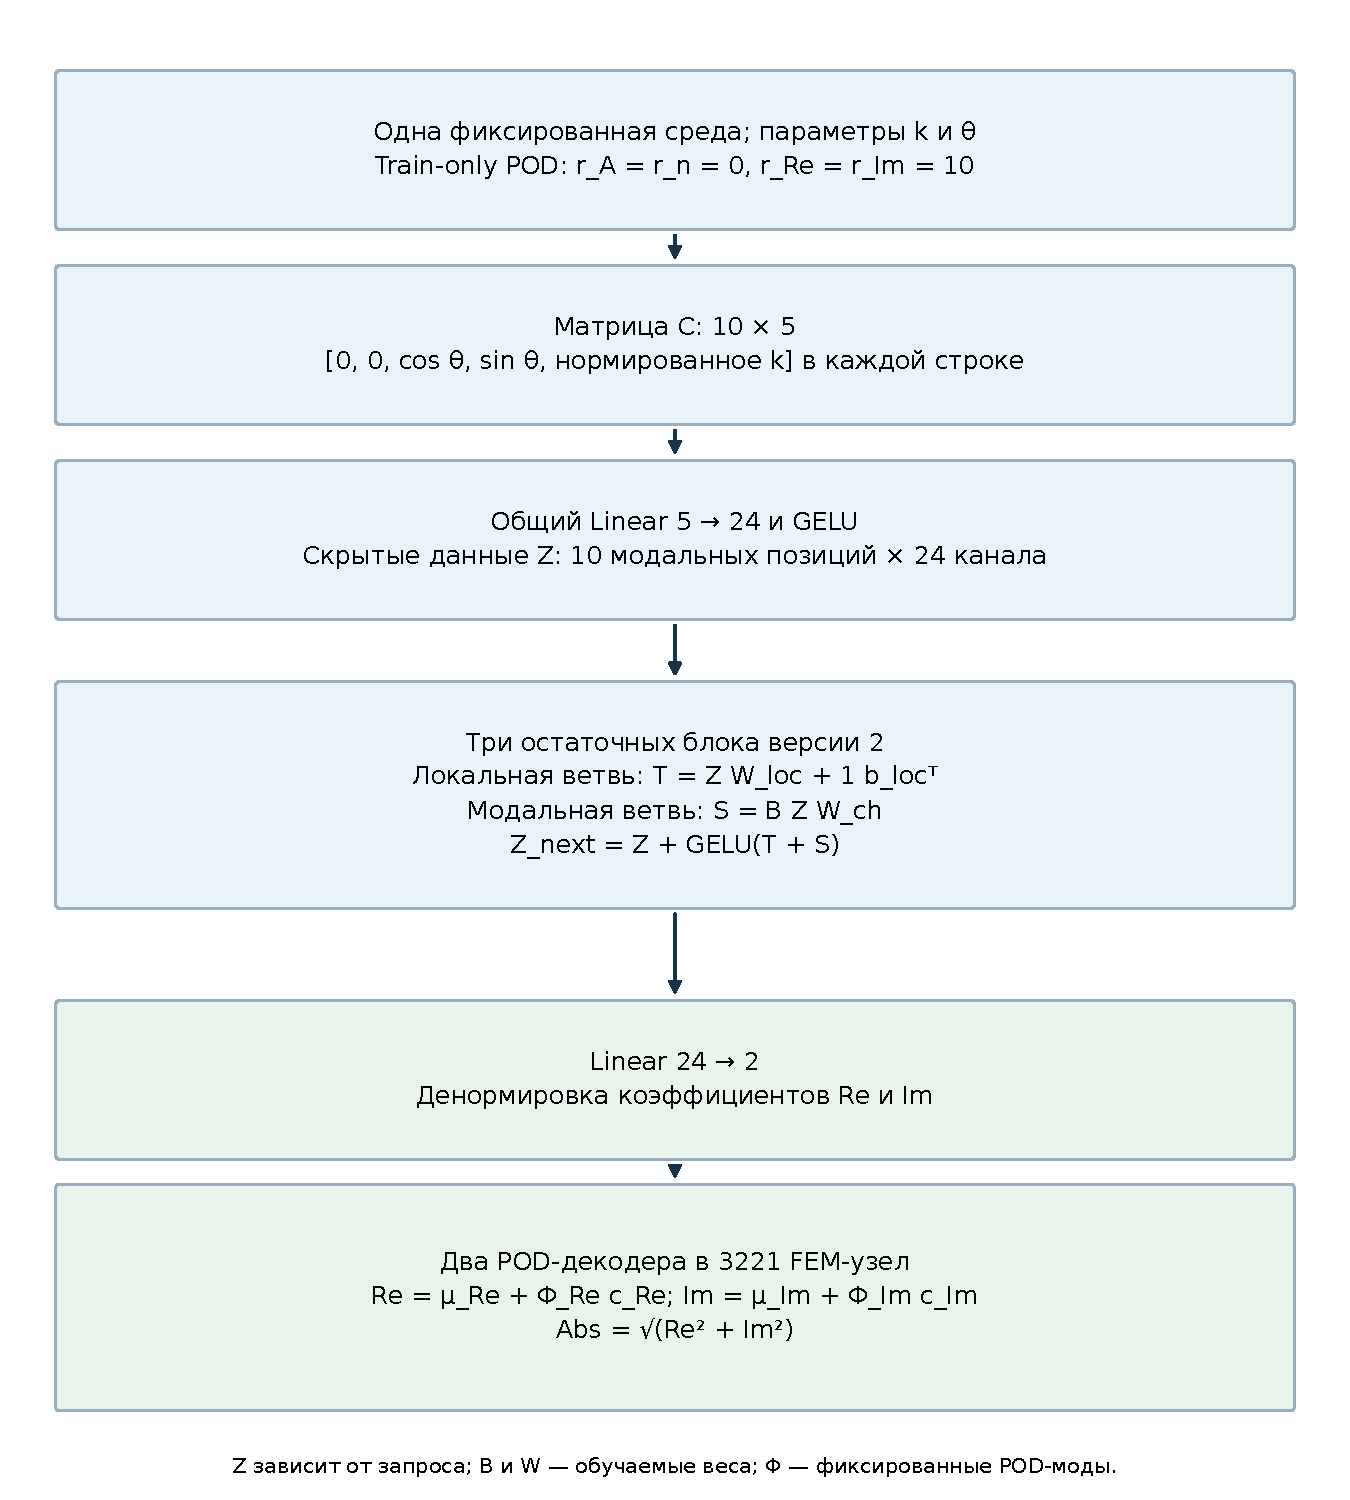
\includegraphics[width=0.95\linewidth,height=0.79\textheight,keepaspectratio]{images/sno_v2_architecture.pdf}
\caption{SVD-SNO версии 2 в текущем статическом примере. Вход содержит параметры волны и два нулевых материальных столбца. Три блока преобразуют модальные признаки; пространственная реконструкция выполняется после предсказания коэффициентов.}
\label{fig:sno}
\end{figure}

\subsection{Согласованный loss в POD-координатах}
Ортогональность~\eqref{eq:pod} относится к \(W\), поэтому реконструкция~\eqref{eq:pod_encode} не обязана минимизировать ошибку в норме \(M\). Для одного компонента определим
\begin{equation}
G=\Phi^\trans M\Phi,\quad
\bm c_*=G^{-1}\Phi^\trans M(\bm f-\bm m),\quad
\bm\rho=\bm f-\bm m-\Phi\bm c_*.
\label{eq:consistent_projection}
\end{equation}
Тогда
\begin{equation}
\|\bm f-\bm m-\Phi\widehat{\bm c}\|_M^2
=(\widehat{\bm c}-\bm c_*)^\trans G(\widehat{\bm c}-\bm c_*)+\|\bm\rho\|_M^2.
\label{eq:quadratic}
\end{equation}
Сумма выражений Re и Im даёт комплексный числитель~\eqref{eq:metric}. Коэффициенты сети предварительно денормируются, а остаток интегрируется напрямую. Поэтому обучение может вычислять ту же FEM-ошибку через малые Gram-матрицы без восстановления всех узлов в каждом пакете. Лишь согласованная проекция с \(\bm c_*\) задаёт строгий минимум на том же аффинном пространстве для нормы \(M\).

\section{FNO И CHEBYSHEV-SNO}
\subsection{FNO: преобразование Фурье и пространственная нелинейность}
FNO получает семь каналов \((A,n,\cos\theta,\sin\theta,k,x,y)\) на равномерной сетке \(32\times32\). Материалы и частота нормируются по train, координаты масштабируются в \([-1,1]\). FEM-поля переносятся на сетку по барицентрическим весам треугольников. Линейный слой даёт 24 скрытых канала; справа и снизу добавляется по восемь нулевых точек.

Каждый из трёх блоков вычисляет
\begin{equation}
v_{\ell+1}=v_\ell+\sigma\!\left(
\mathcal F^{-1}\{R_\ell(q)\mathcal Fv_\ell(q)\}+L_\ell v_\ell+b_\ell\right).
\label{eq:fno}
\end{equation}
\(L_\ell\) --- свёртка \(1\times1\), \(R_\ell(q)\) --- обучаемые комплексные веса спектральной ветви. В rFFT сохраняются восемь положительных и восемь отрицательных позиций первой оси и восемь неотрицательных позиций второй. GELU действует на значения пространственных признаков после обратного FFT~\cite{li2020}. После удаления padding проекция выдаёт два канала; билинейная интерполяция возвращает их в FEM-узлы, затем применяются train-среднее поле и масштабы компонентов.

Padding не навязывает условие~\eqref{eq:boundary}; сеть обучается граничному поведению по FEM-меткам. Пространственная нелинейность может создавать дополнительные частоты, поэтому FNO не ограничена тем же конечным выходным полиномиальным пространством, что Chebyshev-SNO. В модели 445\,010 вещественных степеней свободы: один комплексный вес считается за два. Схема приведена на рис.~\ref{fig:fno}.

\begin{figure}[p]
\centering
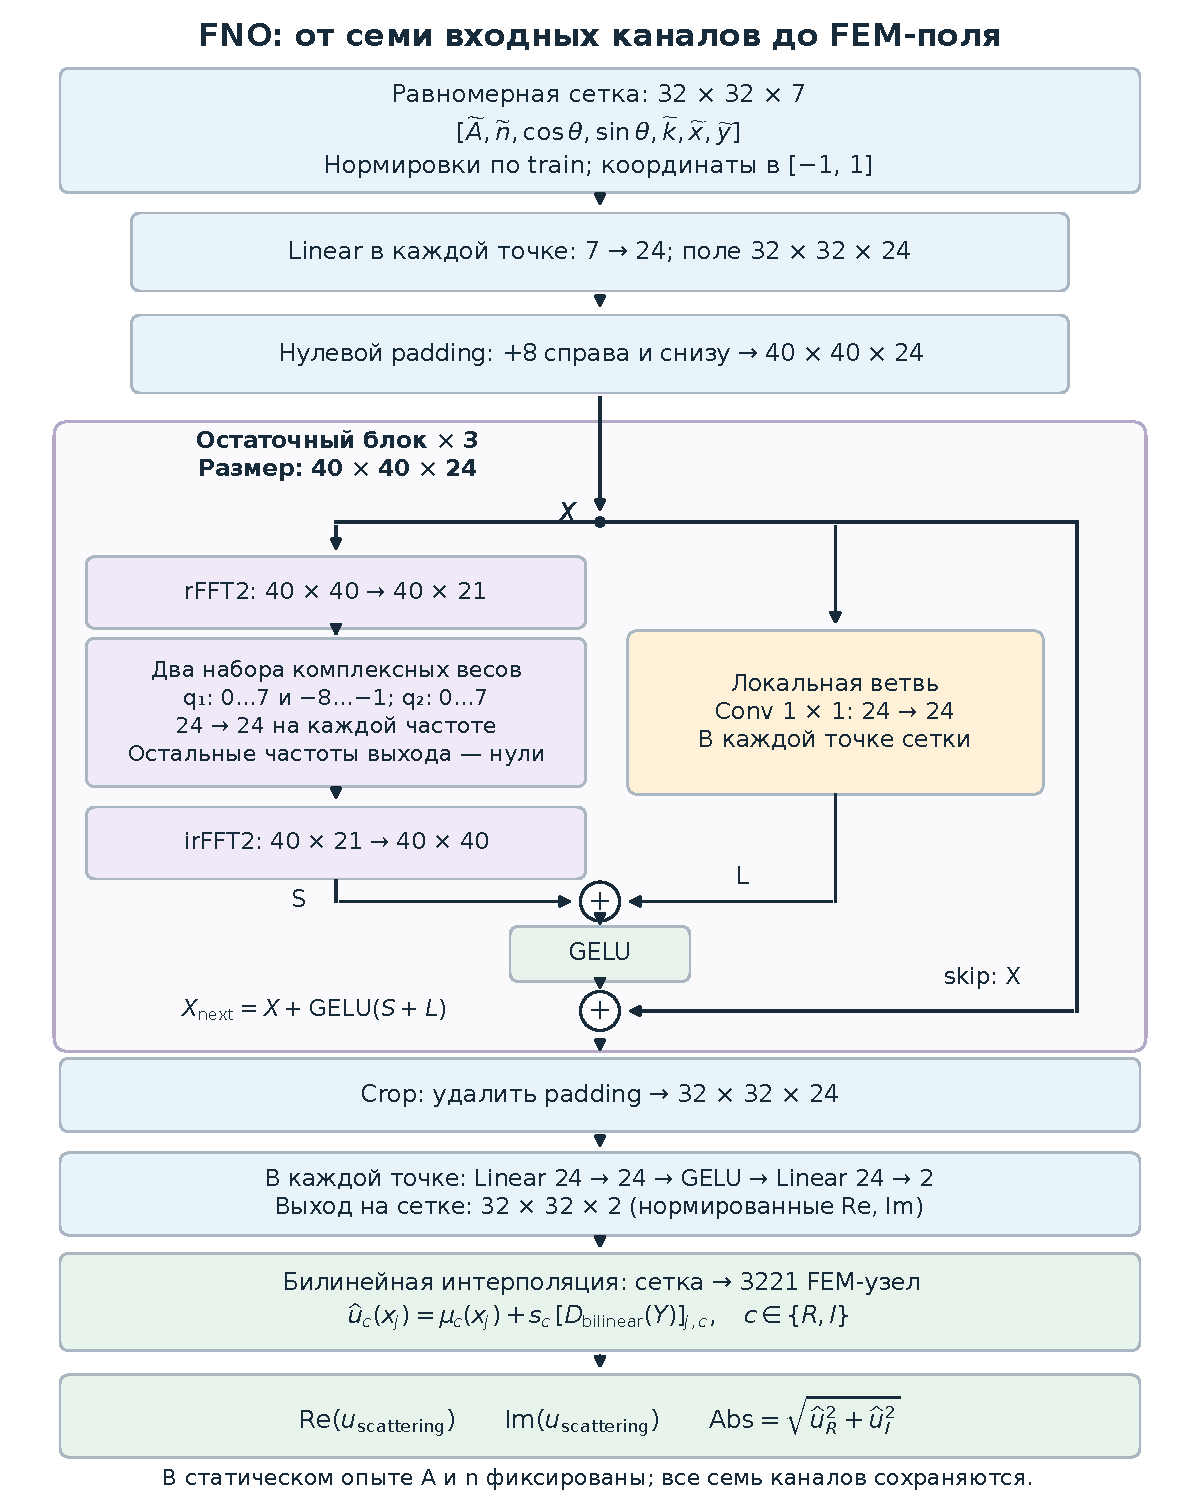
\includegraphics[width=0.95\linewidth,height=0.79\textheight,keepaspectratio]{images/fno_architecture.pdf}
\caption{FNO текущей конфигурации. Спектральная и локальная ветви обрабатывают пространственные признаки. Итоговое поле восстанавливается в исходных FEM-узлах; модуль определяется по Re и Im. Размеры показаны без оси пакета.}
\label{fig:fno}
\end{figure}

\subsection{Chebyshev-SNO: тензорный базис и DCT-I}
Положим \(\xi=x/2\), \(\eta=y/2\). Фиксированные пространственные функции равны
\begin{equation}
\psi_{ab}(x,y)=T_a(\xi)T_b(\eta),\qquad T_a(\cos t)=\cos(at).
\label{eq:chebyshev}
\end{equation}
На каждой оси берутся 32 узла Лобатто в возрастающем порядке,
\(\xi_j=\cos(\pi(1-j/(m-1)))\), \(m=32\). Для \(S_{ja}=T_a(\xi_j)\) и диагональной \(D\) с крайними значениями \(1/2\) и остальными 1 преобразование DCT-I имеет вид
\begin{equation}
\mathcal A=\frac{2}{m-1}DS^\trans D,\qquad
C=\mathcal A F\mathcal A^\trans,\qquad F=SCS^\trans.
\label{eq:dct}
\end{equation}
Последнее равенство точно восстанавливает значения в узлах при сохранении всех мод. Например, при \(m=3\) значения \(T_2\) в узлах \((-1,0,1)\) равны \((1,-1,1)\), а коэффициенты в принятой записи ряда --- \((0,0,1)\). Этот пример фиксирует нормировку крайних коэффициентов.

В расчёте оставляются \(8\times8\) мод семи входных каналов. Линейный подъём даёт массив \(8\times8\times24\). Три остаточных блока смешивают каналы и последовательно обе модальные оси; затем применяются GELU и остаточное сложение. Проекция в два канала и синтез~\eqref{eq:dct} восстанавливают поля на тензорной сетке. Число параметров равно
\begin{equation*}
(7\cdot24+24)+3\bigl(24^2+24+2\cdot8^2\bigr)+(24\cdot2+2)=2426.
\end{equation*}
В отличие от FNO, нелинейность применяется к коэффициентам ряда~\cite{fanaskov2022}. В отличие от POD, пространственные функции не выбираются по снимкам решения.

Перенос FEM\(\to\)Lobatto выполняется барицентрической интерполяцией, обратный перенос --- билинейной. DCT-I не применяется к произвольному индексу неструктурированного FEM-узла. Даже при точном преобразовании остаются ошибки интерполяции и усечения. Для фактической матрицы выходного декодера \(\Psi\), включающей обратный перенос в FEM-узлы, можно вычислить оптимальную согласованную проекцию по~\eqref{eq:consistent_projection} с заменой \(\Phi\) на \(\Psi\). Она измеряет ограничение именно используемого аффинного выходного пространства, а не одного непрерывного полиномиального ряда.

\section{ПРОТОКОЛ ОБУЧЕНИЯ И РЕЗУЛЬТАТЫ}
Для трёх моделей заданы width=24, depth=3, batch=32, seed 42 и максимум 200 эпох. Используется AdamW с шагом 0,002, weight decay \(10^{-5}\) и ограничением глобальной нормы градиента до 1. После каждой эпохи вычисляется средняя validation FEM-ошибка. Итоговое состояние выбирается только по её минимуму; остановка возможна после 50 эпох без улучшения при минимуме 50 эпох. Тест не участвует в выборе состояния сети.

SVD-SNO и Chebyshev-SNO обучены на CPU, существующая FNO --- на Apple M4/MPS; сохранённая FNO повторно проверена на CPU. Одинаковые ширина, глубина и предел эпох не задают одинаковую ёмкость или вычислительный бюджет. Времена этих отдельных запусков не используются для вывода об ускорении.

\begin{table}[htbp]
\centering
\caption{Текущие модели одной среды: ошибки на 1280 удержанных полях, \%; число вещественных параметров}
\label{tab:results}
\begin{tabular}{@{}lrrrrr@{}}
\toprule
Метод & Параметры & Средняя & Медиана & p95 & Максимум\\
\midrule
SVD-SNO v2 & 4\,022 & 0,9475 & 0,8671 & 1,6534 & 2,8962\\
FNO & 445\,010 & 1,6599 & 1,6329 & 1,9505 & 2,2305\\
Chebyshev-SNO & 2\,426 & 7,9364 & 7,6838 & 9,8811 & 11,1065\\
\bottomrule
\end{tabular}
\end{table}

SVD-SNO выполнила 165 эпох, лучшее состояние получено на эпохе 115; FNO --- 142 эпохи с лучшей 92; обе остановлены по validation plateau. Chebyshev-SNO выполнила 200 эпох, лучшее состояние --- эпоха 199; достижение лимита не доказывает сходимость.

На тестовых полях оптимальная согласованная POD-проекция даёт среднюю ошибку 0,9188\%. Она близка к ошибке SVD-SNO, но вычисляется с использованием истинного поля и не является самостоятельным предсказателем. Для фиксированного Chebyshev-декодера с \(8\times8\) модами средняя оптимальная \emph{валидационная} ошибка равна 7,6143\%, p95 --- 9,5266\%. Поэтому одно изменение весов сети при неизменном декодере не может обеспечить среднюю validation-ошибку 1\%. Эта диагностика относится к выбранным модам, сетке и переносу; она не является общим пределом полиномов Чебышёва.

Таблица~\ref{tab:results} сравнивает конкретные зафиксированные запуски. Она не устанавливает универсального ранжирования архитектур: различаются число параметров и представления, а разброс по seed не оценивался. Восемь направлений одной частоты зависимы; 1280 полей соответствуют 160 частотным группам. Доверительные интервалы по группам отдельно не рассчитывались.

\subsection{Один общий пример поля}
Для визуального сравнения используется один и тот же тестовый индекс у всех трёх методов. Выбор выполняется по сохранённому списку test до просмотра ошибок моделей: берётся его первая позиция. Выбран индекс 8: \(k=1{,}001001\), \(\theta=0{,}033124\) рад. Индивидуальные комплексные FEM-ошибки SVD-SNO, FNO и Chebyshev-SNO равны соответственно 1,6985\%, 2,1097\% и 10,9141\%. Точные параметры и ошибки записываются в provenance рисунка. Это конкретный воспроизводимый запрос, а не утверждение о среднем или медианном качестве всей выборки.

На рис.~\ref{fig:predictions_sno}--\ref{fig:predictions_chebyshev} показаны действительная часть, мнимая часть и модуль рассеянного поля. Для каждой компоненты FEM и все три предсказания имеют общие цветовые пределы; шкалы абсолютных ошибок также общие между методами. Ошибка модуля \(\bigl||\widehat u_s|-|u_s|\bigr|\) отличается от комплексной ошибки \(|\widehat u_s-u_s|\), которая лежит в основе~\eqref{eq:metric}. Табличные ошибки не заменяются ошибками выбранной картинки.

\begin{figure}[p]
\centering
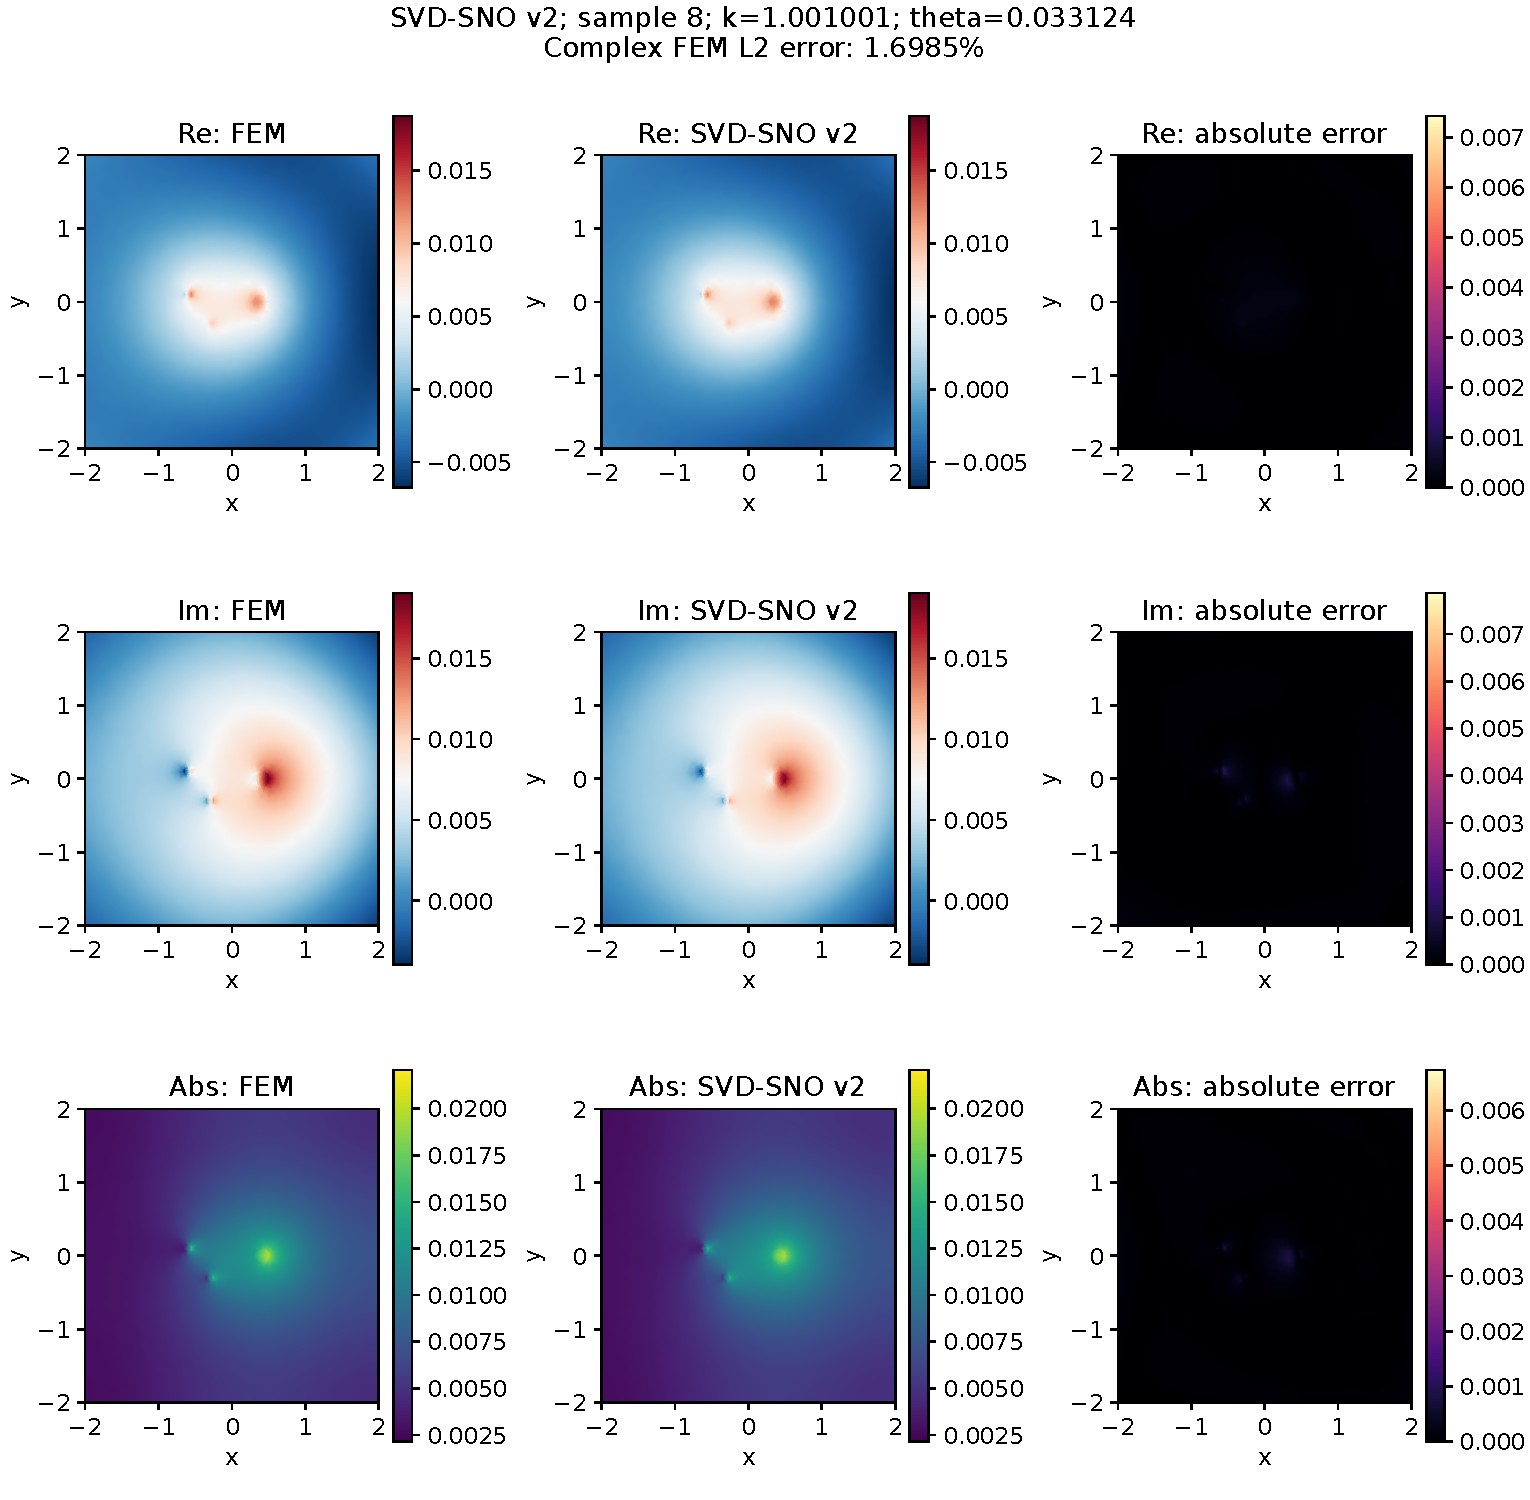
\includegraphics[width=0.95\linewidth,height=0.78\textheight,keepaspectratio]{images/static_low_sno_components.pdf}
\caption{Один общий тестовый запрос: FEM и SVD-SNO v2. Строки: Re, Im и Abs рассеянного поля; столбцы: FEM, предсказание и абсолютная ошибка компоненты. Индивидуальная комплексная FEM-ошибка указана над полями; шкалы согласованы между тремя моделями.}
\label{fig:predictions_sno}
\end{figure}

\begin{figure}[p]
\centering
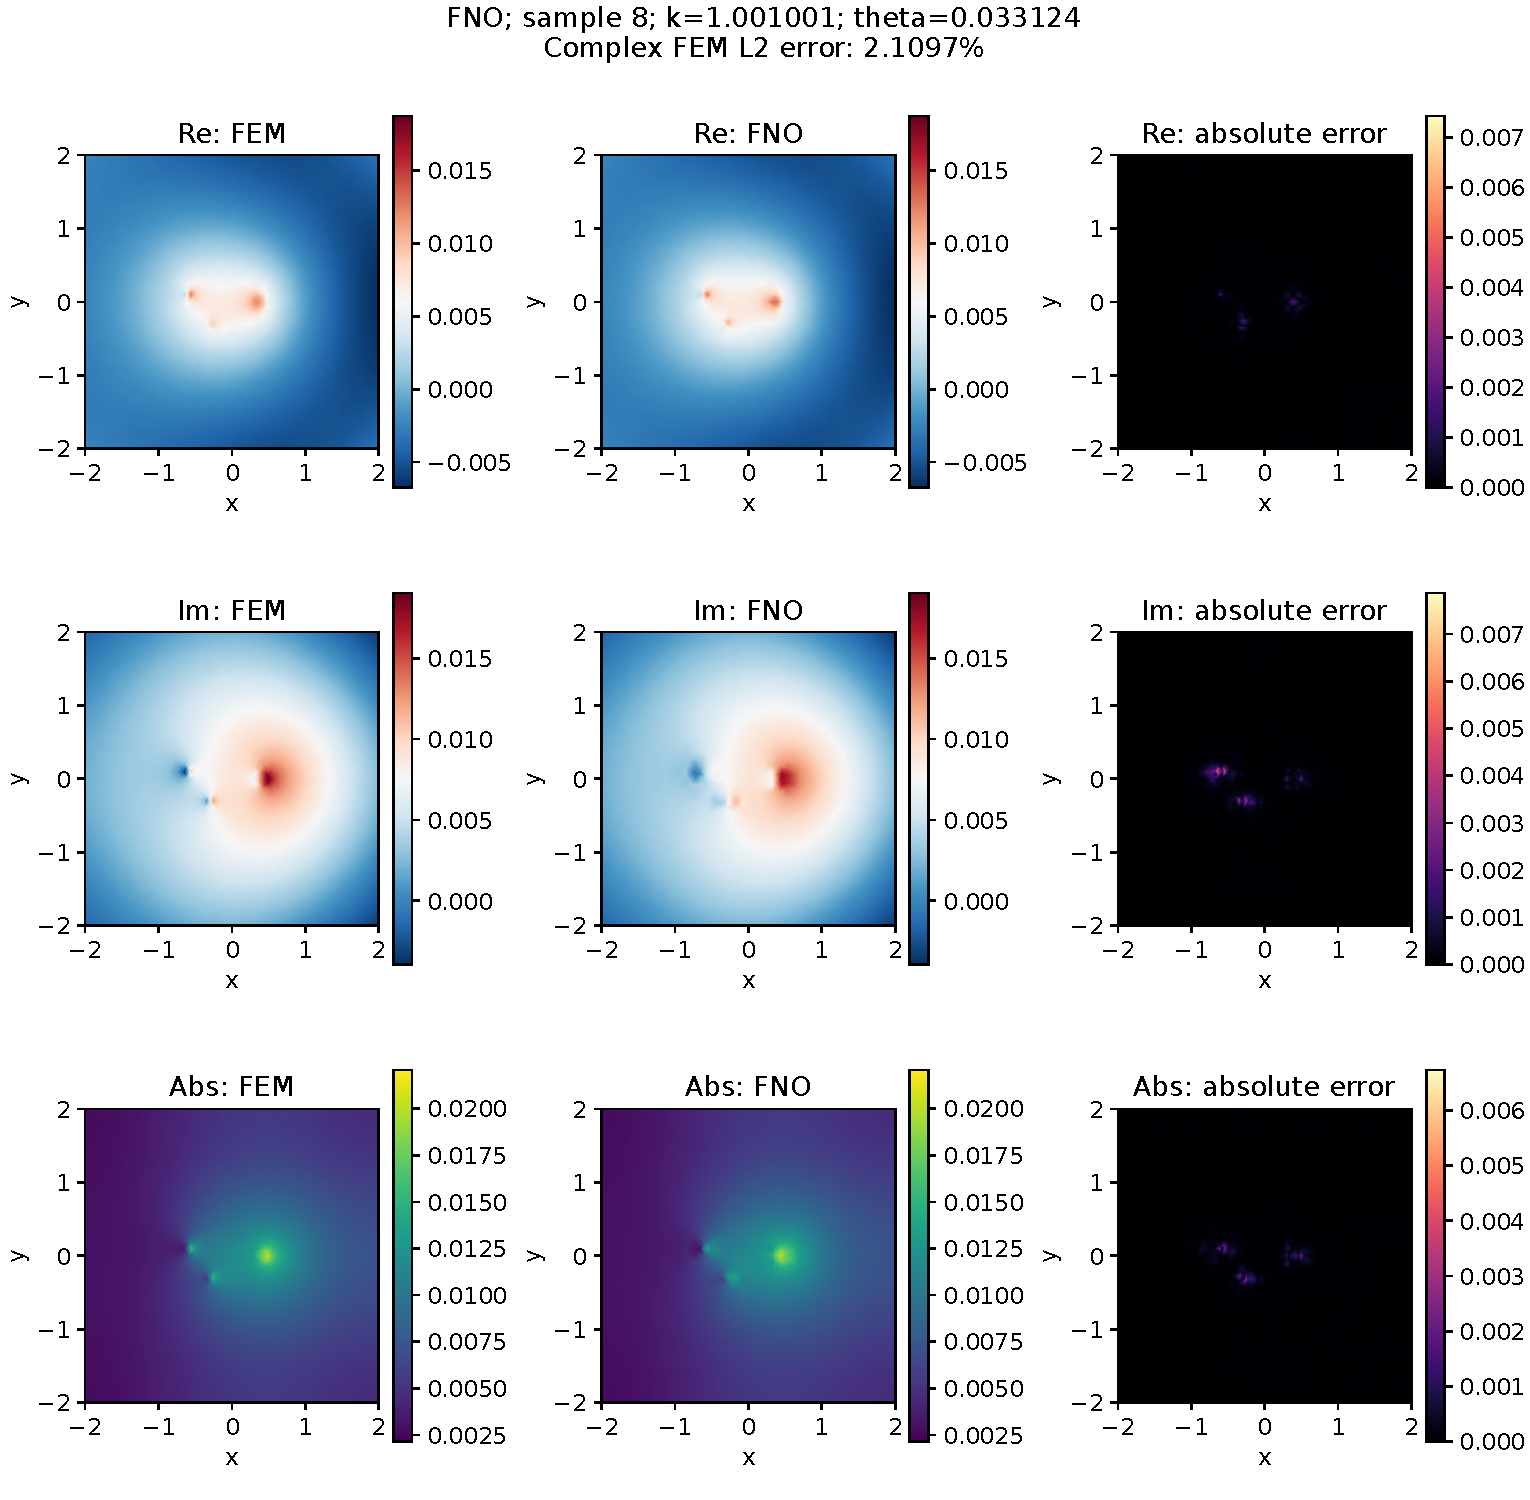
\includegraphics[width=0.95\linewidth,height=0.78\textheight,keepaspectratio]{images/static_low_fno_components.pdf}
\caption{Один общий тестовый запрос: FEM и FNO. Строки: Re, Im и Abs рассеянного поля; столбцы: FEM, предсказание и абсолютная ошибка компоненты. Индивидуальная комплексная FEM-ошибка указана над полями; шкалы согласованы между тремя моделями.}
\label{fig:predictions_fno}
\end{figure}

\begin{figure}[p]
\centering
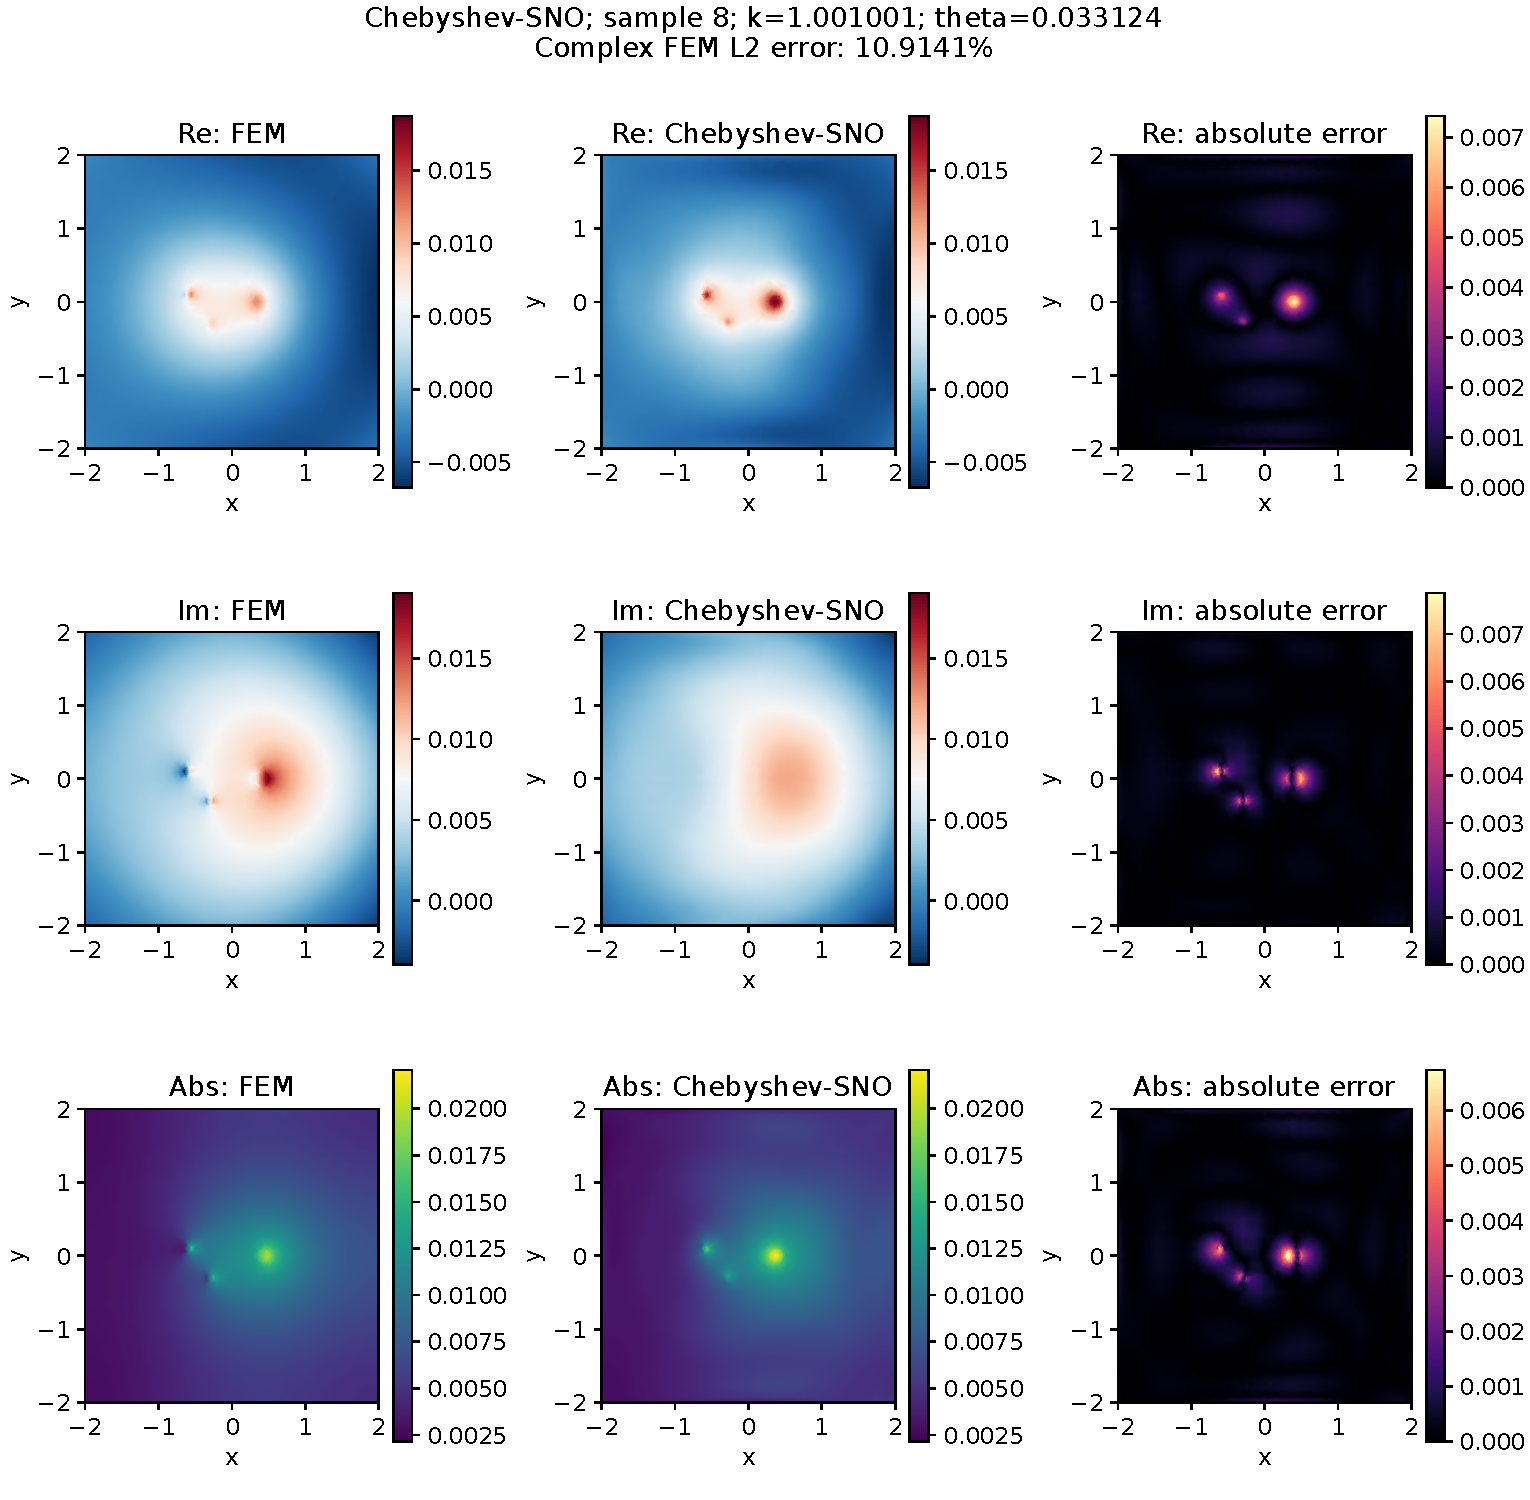
\includegraphics[width=0.95\linewidth,height=0.78\textheight,keepaspectratio]{images/static_low_chebyshev_components.pdf}
\caption{Один общий тестовый запрос: FEM и Chebyshev-SNO. Строки: Re, Im и Abs рассеянного поля; столбцы: FEM, предсказание и абсолютная ошибка компоненты. Индивидуальная комплексная FEM-ошибка указана над полями; шкалы согласованы между тремя моделями.}
\label{fig:predictions_chebyshev}
\end{figure}

\subsection{Воспроизводимость}
Все результаты относятся к одному набору данных, однозначно заданному fingerprint в сопровождающих метаданных.
Сопроводительный файл \texttt{REPRODUCIBILITY.md} содержит команды обучения и проверки существующих весов. В \texttt{evidence/current\_static\_low/} сохранены точные конфигурации, метрики, хеши и сведения о трёх выбранных запусках. Скрипт \texttt{prepare\_predictions.py} проверяет все 1280 test-индексов и ошибок, сверяет предсказание выбранного запроса с повторным инференсом и строит общий пример без обучения и FEM-решений.

\texttt{validate\_paper.py} проверяет snapshots и численные строки статьи, ссылки на рисунки, LaTeX-метки, DCT-I и число параметров. Версии библиотек сохраняются в метриках; архитектурная версия SVD-SNO --- в checkpoint. Независимый новый запуск должен использовать отдельный выходной каталог и сохранять тот же рецепт данных и групповые индексы. Повторение отдельного seed не заменяет исследование устойчивости по нескольким инициализациям.

\section{ЗАКЛЮЧЕНИЕ}
На одной фиксированной среде сопоставлены три способа предсказания комплексного рассеянного поля. При общем частотном разбиении и согласованной FEM-метрике средние тестовые ошибки составляют 0,9475\% для SVD-SNO v2, 1,6599\% для FNO и 7,9364\% для Chebyshev-SNO. Сохранены полные статистики текущих моделей и точные области применимости этих чисел.

POD адаптирует выходное пространство к обучающим полям, а фиксированное полиномиальное представление позволяет отдельно измерить ограничение фактического декодера. Согласованная проекция и loss с Gram-матрицей связывают эти диагностики с той же FEM-нормой, что используется при оценке. Полученные результаты относятся к удержанным частотам \(k\in[1,2]\), одной сетке и одному seed. Проверка новых материалов, других геометрий и точности непрерывной задачи требует самостоятельного протокола.

\begin{thebibliography}{9}
\bibitem{li2020}
Li Z., Kovachki N., Azizzadenesheli K., Liu B., Bhattacharya K., Stuart A., Anandkumar A.
Fourier Neural Operator for Parametric Partial Differential Equations.
ICLR. 2021. \href{https://arxiv.org/abs/2010.08895v3}{arXiv:2010.08895v3}.

\bibitem{fanaskov2022}
Fanaskov V., Oseledets I.
Spectral Neural Operators.
2022; версия 2, 2024. \href{https://arxiv.org/abs/2205.10573v2}{arXiv:2205.10573v2}.

\bibitem{lu2022}
Lu L., Meng X., Cai S., Mao Z., Goswami S., Zhang Z., Karniadakis G.\,E.
A comprehensive and fair comparison of two neural operators (with practical extensions) based on FAIR data.
Computer Methods in Applied Mechanics and Engineering. 2022. Vol.~393. Art.~114778.
\href{https://doi.org/10.1016/j.cma.2022.114778}{doi:10.1016/j.cma.2022.114778}.

\bibitem{halko2011}
Halko N., Martinsson P.-G., Tropp J.\,A.
Finding Structure with Randomness: Probabilistic Algorithms for Constructing Approximate Matrix Decompositions.
SIAM Review. 2011. Vol.~53, No.~2. P.~217--288.
\href{https://doi.org/10.1137/090771806}{doi:10.1137/090771806}.
\end{thebibliography}
\end{document}
